\section*{\large{Motivation}}
\begin{large}
\begin{itemize}
\item Generating agents with \textbf{intelligent-looking} behaviors
has been a constant challenge in the area of Artificial
Intelligence for video games. The user expects to see
agents that can perform \textbf{tactical movements} and
\textbf{group strategies}.

%\item These behaviors tend to be complex in their implementation
%and usually result in pre-established moves that can be easily
%identified by the user.

\item 
A situation that appears frecuently in this area 
is having a group of agennts trying to reach 
 a common target  through pathfinding.
The goal point is usually given by a location in the game map
(potentially the opponent's position).

\item A well known approach is to generate the \textbf{minimal path}
towards the objective.
When the algorithm is executed independently by multiple agents,
it is very likely for the paths to be \textbf{confluent}. Thus,
route diversity and map exploration is prevented.

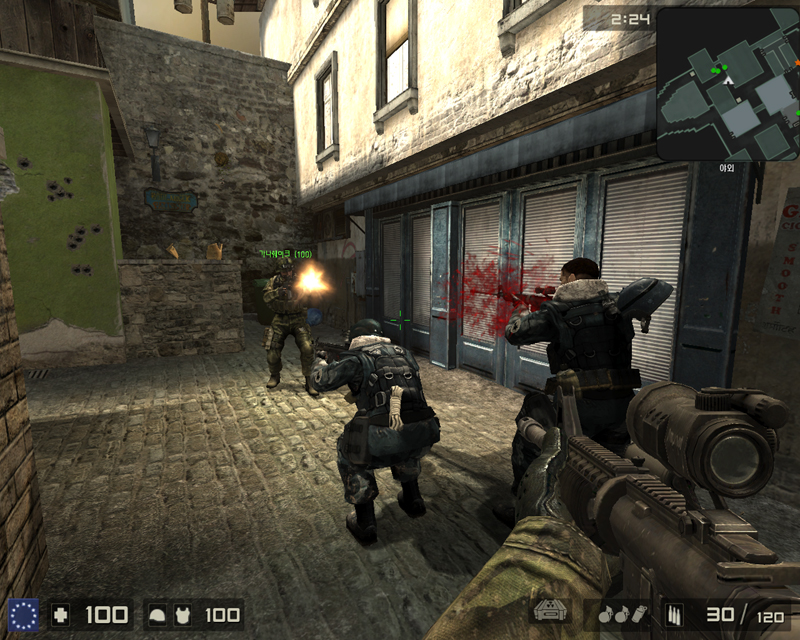
\includegraphics[width=0.15\textwidth, height=10cm]{figures/fps.jpg}
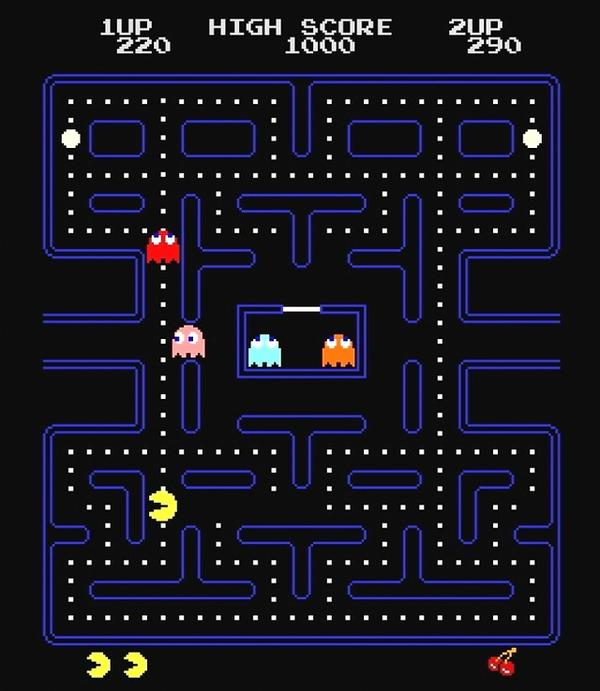
\includegraphics[width=0.15\textwidth, height=10cm]{figures/pacman.jpg}
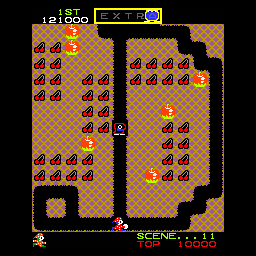
\includegraphics[width=0.15\textwidth, height=10cm]{figures/do.png}

\bigskip
\item When the minimal path strategy is applied for chasing
the enemy, many escape paths are left open. Therefore,
it is of special interest to generate mechanisms of \textbf{route
diversification} that can produce ambush behaviors.
\end{itemize}
\end{large}
